\documentclass[]{article}
\usepackage{a4wide}
\usepackage{xcolor}
\usepackage[numbers]{natbib}
\usepackage[colorlinks,linkcolor=black,urlcolor=blue,citecolor=black]{hyperref}
\usepackage{graphicx}

\newcommand{\TODO}[1]{{\color{red}\textbf{TODO: #1}}}
\newcommand{\reqr}[1]{{\noindent\emph{#1:}}}
\renewcommand*\contentsname{Table of Contents}

\title{Peer Matching Researchverslag}
\author{Marijn Goedegebure \and
	Floris Verburg \and
	Freek van Tienen}
\date{}

\begin{document}
\maketitle

\begin{center}
  \makebox[\textwidth]{
\includegraphics[width=20cm]{Images/MOOCbubble}}
\end{center}

\hfill \textbf{Supervisors:}

\hfill Prof. drs. dr. L.J.M. Rothkrantz

\hfill Dr.ir. D. Datcu


\newpage

\tableofcontents

\newpage

\section{Preface}
This document is the research report that has been written for the Peer Matching assignment for the Bachelor Project course.
This course is the last project based course of the Bachelor of Science at the TU Delft in the Netherlands. The assignment was issued by Prof. drs. dr. L.J.M. Rothkrantz of the TU Delft.
The report provides a summary of the requirements that are set for the system and will provide for a literature study about different possible algorithms to solve the peer matching problem presented in the problem definition.

\section{Introduction}
Many students go to an university each year to follow the predefined bachelor and/or master programs, but not everyone has the time and intent to follow an entire program.
There is a demand from all sorts of people to be able to follow a course while their main occupation isn't that of a student.
For example: a working parent could be very interested in such a course.
That is why universities introduced MOOCs.

The basic idea of MOOCs is that students remote in place and time follow the lectures, can participate in a practical assignment and can make an exam.
If they score sufficient, they are rewarded with a certificate that states their success in the course.

The concept of the MOOCs is a very new concept that still has many areas to improve upon.
One of these areas is the area of practical assignments.
Currently, for a Computer Science MOOC at the TU Delft, multiple practical assignments are required.
The participants are required to form groups to make these assignments.
After the announcement the participants either use mail, Facebook or  Twitter to contact other people in order to form the groups.

TUDelft has been a forerunner in the field of Open \& Online Education since 2007 and is one of the sustaining members of the OpenCourseWare Consortium and since 2013 charter member of the edX Consortium. 
In March 2014, the board of the TU Delft approved an innovation program to accelerate the development of open \& online education. 
The goal is to create a Delft Extension School that will bundle all open \& online courses for a global population of life long learners.

We would like to improve upon this concept and try to provide a more fitting approach.

\subsection{Problem definition}
In this subsection we will continue on the case provided by the introduction.
We will pinpoint the points we would like to improve upon.\\

MOOCs around the world are growing in size and thus the practical assignments need to be easy to manage.
The growth also means that it is more difficult for each participant to find a possible practical partner due to the large amount of people.
It also becomes really difficult to find the correct partner or group members when you don't see each other during courses and haven't even met most of the people from your course.

Most of the time participants of MOOCs are searching group members on social media like Facebook or Twitter.
They just try to look through some of the participants names in the course, search for them on-line through social media and check if they are a capable partner or group member.
This approach takes a lot of time and most of the time there are too much MOOC participants to go trough all of them.

Next to the fact that this process is very time consuming for every participant, it also leads to a sub optimal solution.
This sub optimal solution will be focussed on a group or set of partners which share the same interest and this doesn't say anything if they would form a good group.

We would like to improve upon this process by creating an application that can be used to create practical groups without the participants being required to go search intensively.
Participants should be able to easily access the application, fill in some relevant information about themselves and then be recommended possible group members.
Our peer matching tool is an add on for the MOOCs. 
It can be parallel used for every MOOC with group assignments.
The teacher can create a course in our tool to represent a MOOC.

The interaction with the system is a pretty straight forward application, but the recommendation of possible group members is more difficult.
One of the questions we are trying to answer is: What user information is useful to determine whether two people can be good practical partners?
We will also need to figure out a good way to recommend a practical partner, but still give the possibility to reject such a request.\\

\emph{We have two problems. First, how can we find appropriate matches for people? And second, how can we create optimal groups?}\\

These questions and difficulties will be answered in this report.

\section{Introduction to requirements}
The following sections will describe what requirements are set for the product.
This section will define four global requirements who cover the entire project.
These requirements are then split up in the next two sections, the first being the requirements for the basic system and the second being the requirements for the peer matching algorithm.
We choose to split these requirements up, because of the literature study required to further specify the requirements.
In these sections, the global requirements are split up in smaller requirements.
It is easier to verify these smaller requirements for their completion and these requirements are more transformable to functions of the system.
We also assigned these requirements into their appropriate MoSCoW \cite{highsmith2001agile} method category.

\subsection{Actors of the system}
In this subsection we will clarify the different actors used in the system and throughout this report.
\subsubsection{MOOC participant}
Due to the nature of the MOOCs, there are no requirements set for the participants.
Every person with an interest in the given course can enlist for the MOOC and should thus be able to register with our system.
\subsubsection{MOOC teacher/MOOC administrator} 
The MOOC is organised by a professor of an university.
This professor will need to register with the system and create a MOOC.
\subsubsection{Groups of participants}
This actor consist of two or more MOOC participants who accepted each other to their group.
These groups can be of variable size, set by the MOOC organiser.

\subsection{Global Requirements}
To provide an overview of what the software must be capable of, we define four global requirements for the system.
By defining these four global requirements we provide a foundation of what the system must be able to do.
\begin{itemize}
\item  MOOC teachers must be able to create, manage and edit courses.
Participants of their MOOC are able to register to this course.

\item MOOC students must be able to register and deregister for a course.

\item The system must be capable to use personal data provided by the user to find a suggestion of an appropriate practical partner or group member.
It must be possible to adjust the definition (parameters) of the appropriate practical partner or group member, and search trough several suggestions.
\end{itemize}

\section{Requirements}
This section will mention the different requirements that involve the basic system which the actors interact with.
The section starts with mentioning the possible types of user information the application can use and what requirements are associated with that.
Followed up by what actions are possible within the system.
After that the kind of system is limited by the requirements listed.
Lastly we will list the requirements set for the algorithm.
Each section will use the MoSCoW model to divide the requirements in their appropriate categories.


\subsection{User information}
\reqr{Must have}
\begin{itemize}
\item Users must have a viewable profile that can be filled with personal information.
\item Users must be able to enter the following registration information during registration: Full name, Email address, Password and Language.
\item Users must fill in their academic performances. Which knowledge, skills and completed courses does the user have?
\end{itemize}

\reqr{Should have}
\begin{itemize}
\item Users should be able to enter the basic user information, like: country, age, short description, skills, education, a picture and personality traits.
\end{itemize}

\reqr{Could have}
\begin{itemize}
\item Users could be able to use a personality test to determine their personality traits.
\item Users could be able to fill in their personality traits.
\item Users could be able to enter the following extended user information: preferred group role, role of the other group members, etcetera.
\item Users could be able to enter a predefined questionnaires.
\end{itemize}

\reqr{Would have}
%\begin{itemize}
%\item
%\end{itemize}

\subsection{Usage of the system}

\subsubsection{Actor 1: MOOC participant}

\reqr{Must have}
\begin{itemize}
\item The a potential participant (anyone who visits the site) must be able to view the different MOOCs without registering or logging in.
\item The participant must be able to inform him/herself about the usage of the application without registering or logging in.
\item The participant must be able to register to the application.
\item The participant must be able to log in to the application.
\item The participant must be able to register to the MOOCs which they were enlisted for (known to the administrator).
\item The participant must be able to view a possible practical partner.
\item The participant must be able to communicate with the possible practical partner to verify the matching.
\item The participant must be able to accept or decline the practical partner into his practical group.
\item The participant must be able to communicate within the group.
\end{itemize}

\reqr{Should have}
\begin{itemize}
\item The participant should be able to ask a currently existing group if he can join them.
\item The participant should be able to use their Linkedin profile to log in to the application.
\item In case the participant already has an account, the participant should be able to add the course to his profile using the teachers url.
\item The participant should be able to receive an invitation from a group.
\item The participant should be able to accept the invitation from a group.
\end{itemize}

\reqr{Could have}
\begin{itemize}
\item The participant could be able to set his preferences for his possible partner.
\item The participant could be able to search for other participants using information that is available in the profile.
\end{itemize}

\reqr{Would have}
%\begin{itemize}
%\item
%\end{itemize}


\subsubsection{Actor 2: MOOC teacher/MOOC administrator}
\reqr{Must have}
\begin{itemize}
\item The administrator must be able to create a course and add this to his account.
\item The administrator must be able to open and close the participant registration for a course.
\item The administrator must be able to manage the list of participants and groups of participants.
\item The administrator must be able to create an url that he can use to invite the participants.
\end{itemize}

\reqr{Should have}
\begin{itemize}
\item The administrator should be able to set a deadline for a practical.
\item The administrator should be able to communicate with every participant.
\item The administrator should be able to communicate with the groups.
\end{itemize}

\reqr{Could have}
\begin{itemize}
\item The administrator should be able to grade the group for its practical.
\item The administrator could be able to provide for his own criteria for each of his course.
\item The administrator could be able to add different assignments to the application.
\item The administrator could be able to view what groups have finished what assignments.
\item The administrator could be able to grade the different assignments.
\item The administrator could be able to provide feedback for the different assignments.
\end{itemize}

\reqr{Would have}
%\begin{itemize}
%\item
%\end{itemize}


\subsubsection{Actor 3: Groups of participants}
This actor consist of two or more course participants who accepted each other to their group.

\reqr{Must have}
\begin{itemize}
\item The groups must be able to communicate with each other using the application.
\end{itemize}

\reqr{Should have}
\begin{itemize}
\item A group should be able to view a possible group member.
\item A group should be able to invite a possible group member to join their group.
\item A group should be able to accept an request from a participant to join their group.
\end{itemize}

\reqr{Could have}
\begin{itemize}
\item The group could be able to select their preferences for the new group member.
\item The participants could be able to share files to other group members using this application.
\end{itemize}

\reqr{Would have}
\begin{itemize}
\item The participants would be able upload their source code to the application for verification.
\end{itemize}

\subsection{Kind of system}

\reqr{Must have}
\begin{itemize}
\item The application must be easily accessible to both participants and course organizers.
\item The system must provide account management functionality.
\item The system must use a database to store the different data put in by the user.
\end{itemize}

\reqr{Should have}
%\begin{itemize}
%\item
%\end{itemize}

\reqr{Could have}
\begin{itemize}
\item The system could be able to be combined with practical systems already used by MOOC organizers.
\end{itemize}

\reqr{Would have}
%\begin{itemize}
%\item
%\end{itemize}

\subsection{Peer matching}
\reqr{Must have}
\begin{itemize}
\item The algorithm must be able to use a list of users as input.
\item The algorithm must deal with continuous variation in amount of users.
\item The algorithm must be able to return one or more suggestions of practical partners to the user given a list of rejected users.
\item The algorithm must be able to return one or more suggestions of possible groups the participant could join.
\end{itemize}

\reqr{Should have}
\begin{itemize}
\item The algorithm uses basic user provided data (e.g. education, preferences) to build up a profile for a course participant.
\item The algorithm can calculate whether two people will be good practical partners using the basic user provided data.
\item The algorithm can return a possible practical partners using the basic user provided data.
\end{itemize}

\reqr{Could have}
\begin{itemize}
\item The algorithm uses advanced user provided data (e.g. asked questions, programming tests) to build up an extended profile for a course participant.
\item The algorithm can calculate whether two people will be good practical partners using the advanced user provided data.
\item The algorithm can return a possible practical partner using the basic user provided data.
\item The algorithm could be able to respond to the preferences of groups.
\item The algorithm could be able to respond to the preferences of a participant.
\end{itemize}

\reqr{Would have}
\begin{itemize}
\item The algorithm would have to be able to use information gathered from rejections to improve the matching.
\end{itemize}

\section{Design choices}
In this section we will be describing our choices for the design.
For each choice we will be arguing why we have chosen for this.
We will argue using scientific literature or the requirements.
We will first describe the choices we have made concerning the kind of system.
Secondly we will describe the choices we have made concerning the framework that we will be using.
Following this, we will be describing the choices we have made concerning the algorithm.

\subsection{Global system design}
In the global system design we will be describing a first concept of the system.
In this concept we will describe the different actions, that different actors will need to be able to perform.

The first thing that has to be done is for the teacher to create an assignment in the application.
It must be possible for the teacher to open and close this assignment. 
While creating, the teacher has to define some properties of the assignment.
When the assignment is created successfully, a link is generated that can be sent to the students.

When the students open the link, they have a choice between logging in or registering.
For logging in and registering, the student could use LinkedIn, so a lot of data is gathered automatically.
We can also look for LinkedIn alternatives, like Yammer and Ututi, which are non-commercial.
After filling in the basic information, the student must provide information about his personality.
This can be done by means of an questionnaire.

After logging in, the assignment can be added to the profile of the student.
After adding the assignment to the profile, some recommendations are provided.
The student can form groups by means of this recommendations.

\subsection{Web application}
Our main decision about choosing to make a Web application was relatively simple.
This is due to the fact that MOOCs itself are also Web applications, which are available for everyone.
Because our application is specifically designed for MOOCs it should also be widely available for all the MOOC participants.
One of the best ways to do this is by developing a web application.

\subsection{Framework}
Because Web applications are getting more and more popular, a lot of frameworks are appearing which we could use for our Peer Matching system.
Choosing the right framework is there for really difficult, because they are hard to compare and not a good way to say which is better.
We there for listed a couple of frameworks which we had experience with, to make sure we have a lot of knowledge available in our programming team.

\TODO{more frameworks}

The last framework we looked at was the Play Framework\cite{play}, based on the programming language Java and Scala.
Play is a high-productivity Java and Scala web application framework that integrates the components and APIs you need for modern web application development.

\TODO{conclusion}

\subsection{Algorithm}
Using the requirements stated in the previous section we see that the requirements all state the need for the handling of a specific set of input and outputting the needed information.
The requirements do not state any limitations about the inner workings of the algorithm.
Some questions remain:
\begin{itemize}
\item How does the algorithm determine a possible practical partner?
\item How does the algorithm make a difference between two possible partners and determine which one is a better fit?
\item How does the algorithm make use the extra information provided if the could haves are achieved?
\item How does it make sure the partner that is recommended hasn't already been suggested?
\end{itemize}
Due to the unique requirements set to how the system works, we need to look for all kinds of different algorithms that could help us solve our problem.
Because of the unique requirements, these techniques will probably not solve the entire problem, but we can possibly use parts of these algorithms to formulate our own solution.

We have done a literature survey into recommender systems since these kind of systems are closely related to what we want to achieve.

As can be read in these papers \citep{Breese1998},\citep{Peter2007}, there are roughly five kinds of algorithmic recommendation approaches:

\begin{itemize}
\item Demographic filtering \citep{Peter2007}
\item Collaborative filtering \citep{Peter2007}\citep{Breese1998}
\item Content-based filtering \citep{Peter2007}
\item Knowledge-based filtering \citep{Peter2007}\cite{burke2000knowledge}
\item Hybrid filtering \citep{Peter2007}
\end{itemize}

Next to these recommendations we added a subsection for the mentioning of other possibilities that we encountered while researching the subject.

We will now first discuss each of the techniques mentioned above.\\
\makebox[\textwidth]{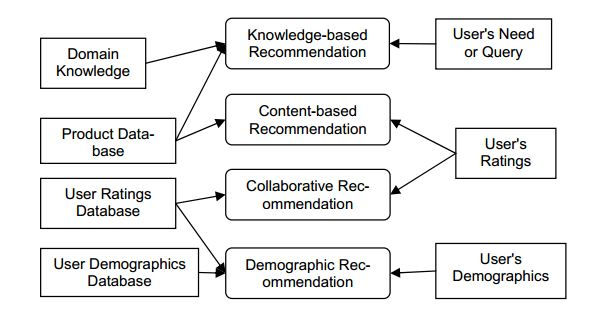
\includegraphics[width=12cm]{Images/RecommendationDomain}}
\TODO{Zeg iets over plaatje}
We will name what aspects are usable and what aspects are not.

\subsubsection{Demographic filtering}
In the paper Privacy-preserving demographic filtering\cite{aimeur2006privacy} demographic filtering is explained.
Recommender systems based on demographic filtering aim at categorising users based on their demographic information and recommend services accordingly. 
More precisely, demographic information is used to identify the types of users that like similar services. 

Demographic filtering can be used by any recommender system that offers services by using data on individual users. 
The key element of demographic filtering is that it creates categories of users having similar demographic characteristics, and tracks the aggregate behaviour or preferences of users within these categories. 
Recommendations for a new user are issued by first finding to which category he belongs and then by applying the aggregate preferences of previous users in that category.

In the paper A framework for collaborative, content-based and demographic filtering\cite{pazzani1999framework} an example is provide. 
For example, Table \ref{table:dfexample}  shows information on the age, gender, education, etc. of people that rated
a restaurant together with their rating of the restaurant. 
One might expect to learn the type of person that likes a certain restaurant. \\ 

\begin{table}[h]
    \begin{tabular}{|l|l|l|l|l|l||l|}
    \hline
    ~     & gender & age & area code & education & employed & Dolce \\ \hline
    Karen & F      & 15  & 714       & HS        & F        & +     \\ \hline
    Lynn  & F      & 17  & 714       & HS        & F        & -     \\ \hline
    Chris & M      & 35  & 714       & C         & T        & +     \\ \hline
    Mike  & F      & 40  & 714       & C         & T        & -     \\ \hline
    Jill  & F      & 10  & 714       & E         & F        & ?     \\ \hline
    \end{tabular}
\caption{Demographic filtering example}
\label{table:dfexample}
\end{table}

\noindent We could use data like these to recommend similar groups for people with the same demographic background.

\subsubsection{Collaborative filtering}
The book Adaptive Web \citep{Peter2007} describes what collaborative filtering techniques are.
He says that these techniques generally involve matching the ratings of a current user for objects with those of similar users.
In this way it produces recommendations for objects that the users has not yet rated or have not been seen by the active user.
Traditionally, the primary technique used to implement a collaborative filtering is the use of k-Nearest-Neighbor (kNN) algorithm.
This algorithm compares a target user's profile with the historical profiles of other users in order to find the top k users who have similar tastes or interests.

Examples of collaborative filtering algorithms are found in the on-line dating branch.
An example that provides some insightful information about the subject is OKCupid.
The video ,that can be found on the website\cite{okcupid}, describes the workings of the OKCupid algorithm.
The OKCupid algorithm uses the geometric mean.
This is a type of mean or average, which indicates the central tendency or typical value of a set of numbers.
OKCupid's algorithm is an algorithm that uses questions and preferences to determine whether two people would make a good pair.
Instead of the questions they ask, we could fill in our own questions or values.
The geometric mean would still give an overall score for the combining of two people.\\

\subsubsection{Content-based filtering}
The book Adaptive Web \citep{Peter2007} also describes what content-based filtering techniques are.
He describes content-based filtering systems as systems where in a user profile represents the content description of items in which that user has previously expressed interest.
The content description of items are represented by a set of features or attributes that characterize that item.
The recommendation in these kind of systems usually consist of comparing unseen or unrated items with the user profile.
Items that overlap with the interests of the user are recommended.

The paper Using Content-Based Filtering for Recommendation \cite{van2000using} describes an example of a recommender system that uses user information to determine what to recommend.\\
In this paper it becomes clear that a built up user profile can give a much better recommendation than a starting profile.
Although this can work for many applications, this means that the user needs to build up a training set.
The first couple of recommendations could be possibly bad and this is not in the users interest.
The user wants the best recommendation from the start.
Although it might look like content-based filtering can not be used for our domain, we would like to keep them in our thought as a possible way to improve upon the algorithm.
By using the user's history we can improve the recommendations by listening more to the users preferences.

\subsubsection{Knowledge-based filtering}
In the book Adaptive Web, they also mentioned knowledge-based filtering as a class of recommendation techniques.
This is supported by a paper called Knowledge-based recommender systems \cite{burke2000knowledge}.
In this paper they describe it as a recommender system that uses knowledge about users and products to generate a recommendation.
It will use this knowledge to have a different approach to the generation of a recommendation and the user.
Knowledge-based recommendation systems do not have the problem of a so called cold-start problem.
The cold-start problem is the problem when a learning-based system does not have enough information to provide for a proper recommendation.
Learning-based systems are systems that learn from each user or product added to the system.
With each step they learn more about the users that are in the system and their preferences.
This can occur when a new user is registered to the system, a new product or when there are only a few current users.
This is a big advantage and is something we should keep in mind when designing our algorithm

One of the downsides of knowledge-based filtering is that it can't learn.
It will always be limited to the knowledge it has.
An expert can improve the knowledge the system has, but it will not do so autonomous like a learning-based system.

\subsubsection{Hybrid filtering}
Adaptive web sites offer recommendations to the user by using a well studied technique.
This technique can either use collaborative, knowledge-based and content-based recommendation, but it can also use a combination of these techniques.
These kind of systems are called hybrid filtering techniques.
Each of these techniques has its own strength and weaknesses and by combining these researchers try to improve the performance of the techniques.
The resulting systems are called hybrid recommender systems and are defined as the combination of two or more of the different recommendation techniques.

A variety of techniques have been proposed as the basis for hybrid recommender systems: collaborative, content-based, knowledge-based and demographic techniques.

The learning-based techniques (collaborative, content-based and demographic) suffer from the cold-start problem.
Most hybrid recommender systems are combining techniques to deal with the cold-start problem.
This is something we need to keep in mind when designing our algorithm.

The converse of this problem is the stability versus plasticity problem.
Once a user's profile has been established in the system, it is difficult to change one's preferences.
Many adaptive systems make the older ratings have less influence and thus prevent the unresponsiveness of the system.

We can use a combination of different techniques, and thus have a hybrid filtering, to have a resulting algorithm that perfectly adheres to the requirements.

\subsubsection{Other possibilities}
Recommender system all try to use data that has been collected to improve their recommendations, but there are other approaches to the matching problem.
A great example of an user based approach is the Tinder mobile-app.
This application allows users to get in contact with other people.
They only provide for a platform where the user can view people who are near you and adhere to some basic requirements (E.g. age limit and amount of kilometres away).
The user is shown a small profile of a potential match and let the user decide whether it is a go or not based on that info.\\
We would like our user to decide upon skills that are not very applicable to the Tinder format.
Another downside of the format is that it does not provide for a way to influence the outcomes of the groups.
For example, the administrator should be able to set values for the different skills that are advised for each group.
Lastly, we would like to narrow down the possible people an user will see to the ones that could be a positive addition to his group.
Although we can not use the entire format, we can use the accepting and/or rejecting of a possible group member.
It is also a good idea to let the possible group members talk to each other before they have to decide to join one's group.

\subsubsection{Conclusion}
Each of these techniques are very interesting for having a good recommendation algorithm, but we do not have the time within this project to expand so vastly on the subject.
We will thus try to simplify the problem to something that we can

\subsubsection{Self assembled algorithm}
\TODO{Herschrijven naar nieuwe setting}\\
\TODO{Toevoegen welke onderdelen worden gebruikt}\\
\TODO{Visualiseren van het algoritme}\\
We concluded that these weren't appropriate for the requirements that were set.
There are three reasons why the techniques mentioned above aren't appropriate for our solution.
First is the fact that the requirements state the need for the administrator to be able to influence the group characteristics.
Secondly the requirements state the possibility that the participants could be able to influence the recommendation.
Lastly not every method is able to easily provide for groups of different sizes.
The techniques mentioned above do not provide for the flexibility 
That is why we took another look at the requirements and how the different actors should interact with each other.
During this evaluation we thought up a algorithm that combines multiple known techniques that adheres to the requirements.

\emph{The algorithm:}\\
The algorithm is centred around the usage of the m properties a participant has to fill in as user information.
These properties will be used to determine whether the combination of two participants results in a combined property that lies closed to a predefined number for this property.
This predefined number can either be set by the administrator or later adjusted by the searching participant.

There are two cases in which the algorithm should be able to recommend a new group member:\\
\emph{A single participant searches for a first group member}
Given m properties and n participants currently enlisted to the course the algorithm will search for a possible practical partner for participant X.
The algorithm determines for each possible practical partner how the creation of a group of that pair would bring them closer to the predefined numbers.
It will do this by taking the average for each property and taking the difference between this average and the predefined number.
It will then sum these differences and take the m root of this number.
This will result in an number that represents the overall difference between the group of the two participants and the predefined numbers.
A group with a low overall difference means that the two participants form a group that as closely meet the predefined numbers as possible.
During this calculation the algorithm keeps track of the top possible practical partners which it will return as a result to the participant.

\emph{A group searches for a new group member}
The second case is similar to the first, the calculation is completely the same.
The only difference is that you do not start with a participant X, but with a group of participants.
The properties of these participants are already averaged per property.
This results in a number per property which can be used by the algorithm mentioned above.

\subsubsection{Possible improvements of the algorithm}
\begin{itemize}
\item The user can use extra properties (which the administrator can't define) to further specify their groups.
\item The user can adjust the predefined numbers (the predefined numbers of the administrator are not required).
\item The algorithm uses the group size to ensure that there are more versatile people in a group.
\end{itemize}

\section{Conclusion}

\newpage
\bibliographystyle{plainnat}
\bibliography{references}

\end{document}